% !TeX spellcheck = ru_RU
% !TEX root = vkr.tex

\section*{Введение}
% Использование линейной алгебры встречается в различных областях: от машинного обучения [ссылочка на статью] до теории графов [ссылочка на статью].
% \begin{enumerate}
%     \item Откуда и почему появляются разряженные матрицы.
%     \item Почему хочется улучшать производительность.
%     \item Почему выбран для этих целей template haskell.
%     \item Что такое kernel fusion.
%     \item Про template haskell
% \end{enumerate}
При работе с большими объёмами данных возникает множество проблем, одна из них~--- промежуточные структуры данных, которые никак не используются в результате, могут давать большую нагрузку на память и замедлять работу программы. Более или менее частные решения этой проблемы существуют: \textit{stream fusion}, дефорестация, суперкомпиляция, дистилляция.

Данные подходы имеют смысл, однако некоторые из них применимы только в крайне специфических областях, например, \textit{Tensorflow} для работы с тензорами, которые нужны для алгоритмов машинного обучения, или наоборот, крайне общие, очень теоретизированные и плохо \enquote{реально} изученные, например, дистилляция.

Таким образом, возникает идея изучения какого-то из наиболее общих методов в каких-то частных случаях для более лёгкого анализа.Слияние ядер~--- один из таких методов, он позволяет уменьшить количество промежуточных структур данных по средствам одновременной обработки узлов. Так как большинство литературы о новейших из этих методов используют модельные языки, имеющие функциональную природу, было решено писать на языке \Haskell{}, а в качестве частного случая рассматривать матрицы, представленные в виде деревьев квадрантов, крайне удобные для обработки в данной парадигме.
% \begin{figure}[ht]
    \centering
    % First minipage
    \begin{minipage}[b]{0.45\textwidth}
        \centering
        \resizebox{\linewidth}{!}{
            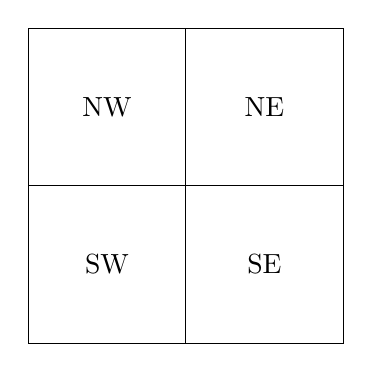
\begin{tikzpicture}
                \draw (1, 1) rectangle (3, 3);
                \draw (1, 3)rectangle (3, 5);
                \draw (3, 1)rectangle (5, 3);
                \draw (3, 3)rectangle (5, 5);
                \node at (2, 2){SW};
                \node at (4, 4){NE};
                \node at (2, 4){NW};
                \node at (4, 2){SE};
            \end{tikzpicture}
        }
        \caption{Квадратная матрица, разделенная на квадранты}
        \label{qmatrix}
    \end{minipage}
    \hfill
    % Second minipage
    \begin{minipage}[b]{0.45\textwidth}
        \centering
        \Tree [.Matrix
                [.NW [] ]
                [.NE [] ]
                [.SW [] ]
                [.SE [] ]
        ]
        \caption{Схематичное изображение одного из узлов дерева квадрантов и его потомков}
        \label{qtree1}
    \end{minipage}
\end{figure}

